\documentclass[12pt]{article} \usepackage{simplemargins}
\usepackage[pdftex]{graphicx} \graphicspath{{figures/}}

\setlength{\parindent}{0pt} \setlength{\parskip}{1.6ex}
\setallmargins{1in} \linespread{1.6}

\begin{document}

\title{A probabilistic framework for scalable assembly graphs}
\author{JP, Arend Hintze, Rosangela Canino-Koning, CTB}

\maketitle

\section{Introduction}

We introduce a fast and lightweight representation of DNA k-mer graphs
based on a probabilistic representation.  This graph has a one-sided
error that is precisely tunable and yields predictable degradation of
graph properties.  We show that this graph representation can be used
to characterize the structure of large assembly graphs.

\section{Results}

\subsection{Storing de Bruijn graphs in Bloom filters}

We can store de bruijn graphs in Bloom filters which gives us a fast and lightweight way to represent them.

\begin{figure}
\center{\includegraphics[width=5in]{figures/f1}}
\caption{Bloom filter.}
\end{figure}

\subsection{Effect of false positives}

This representation has a one-sided error that we can measure and
predict in terms of its impact on graph properties.  Link degradation
to percolation here.

\begin{figure}
\center{\includegraphics[width=5in]{figures/f2b}}
\caption{Bloom filters scale well.}
\end{figure}

\begin{figure}
\center{\includegraphics[width=5in]{figures/f2a}}
\caption{There is a minimum false positive rate for a given amount of memory
and amount of data, set by the number of hash tables.}
\end{figure}


\begin{figure}
\center{\includegraphics[width=5in]{percolation_K5_to_K12_withLegend}}

\caption{K independence, relative size of the largest connected component
$\theta$ for kMer occupancy p (0.0 to 1.0) of various de Bruijn graphs of
different sizes K (5 to 12 see legend), showing the independence of the
percolation threshold ($\theta = 0.5$) from K.
For each datapoint p 1000 random samples were generated keeping the std error
for each datapoint under 0.0047 while the mean std error for all data points is
$< \approx 0.0002$ (data not shown).}
\end{figure}

\begin{figure}
\center{\includegraphics[width=3in]{memoryFraction_vs_percolationThreshold}}
\caption{The critical point for percolation is linearly related to the
  compression factor of the graph representation.
This figure shows
  the interpolated critical percolation threshold dependence on the
  memory used for the Bloom filter. $\rho$ is the fraction of
  maximally required memory ($4^{12}$ bits) for a de Bruijn graph with
  K=12. We reduced the memory allowed $\rho$ from 1.0 to 0.1 (x
  axis). The critical percolation threshold $\theta_{\rm critical}$
  was linearly interpolated (at the critical point $\theta=0.5$ the
  slope is infinite allowing for this). The std deviation is given for
  each interpolation. This plot shows a linear relation between
  allowed memory and expected percolation threshold assuming random
  data. We can fit the following function to this plot: $\theta_{\rm
    critical} = 0.209 \rho + 0.0052$ describing the fraction of memory
  where random data would percolate.  {\bf CTB: this linear result is
    what you'd expect if the slope of the approach to percolation
    across increased occupancy is exponential, given the logarithimic
    false positive rate wrt memory?}}

\end{figure}

\subsection{This can usefully be applied to assembly graphs}

We can use this to look at local assembly graphs usefully.

\paragraph{Fidelity of local graph properties is tunable.}

\begin{figure}
\center{\includegraphics[width=5in]{k31}}
\caption{Approach to critical percolation limit. {\bf Is this an
    exponential?  Or what?  Might be too sharp for that, but what
    would the functional form be? Can we fit?  Do we know the constants?}}
\end{figure}

\paragraph{Large scale graph structure is retained even with high FP rate, out to percolation threshold.}

\begin{figure}
\includegraphics[width=3in]{figures/f3b001}
\includegraphics[width=3in]{figures/f3b005}\\
\includegraphics[width=3in]{figures/f3b010}
\includegraphics[width=3in]{figures/f3b015}
\caption{Decreasing fidelity of graph structure with false positive rate.
{\bf CTB: This should be out first figure, I think!}}
\end{figure}



\paragraph{Both local and large scale graph structure fidelity is preserved for relatively low memory representations.}

\paragraph{We can partition exact data and inexact (error-prone) data.}

\begin{figure}
\center{\includegraphics[width=5in]{figures/f3d}}
\caption{Computation required to partition graphs grows with false positive
rate.  CTB: good to know, but I think this figure can go away; it's implied
by everything else.}
\end{figure}

\paragraph{Link error-prone sequencing to percolation threshold?  Error inflates number of unique k-mers being added in => increases memory requirements.}

Can we discuss sequencing errors for PacBio and link to percolation (show
that even reasonably high sequencing error rate would not percolate?)

100x coverage issue.

\begin{figure}
\center{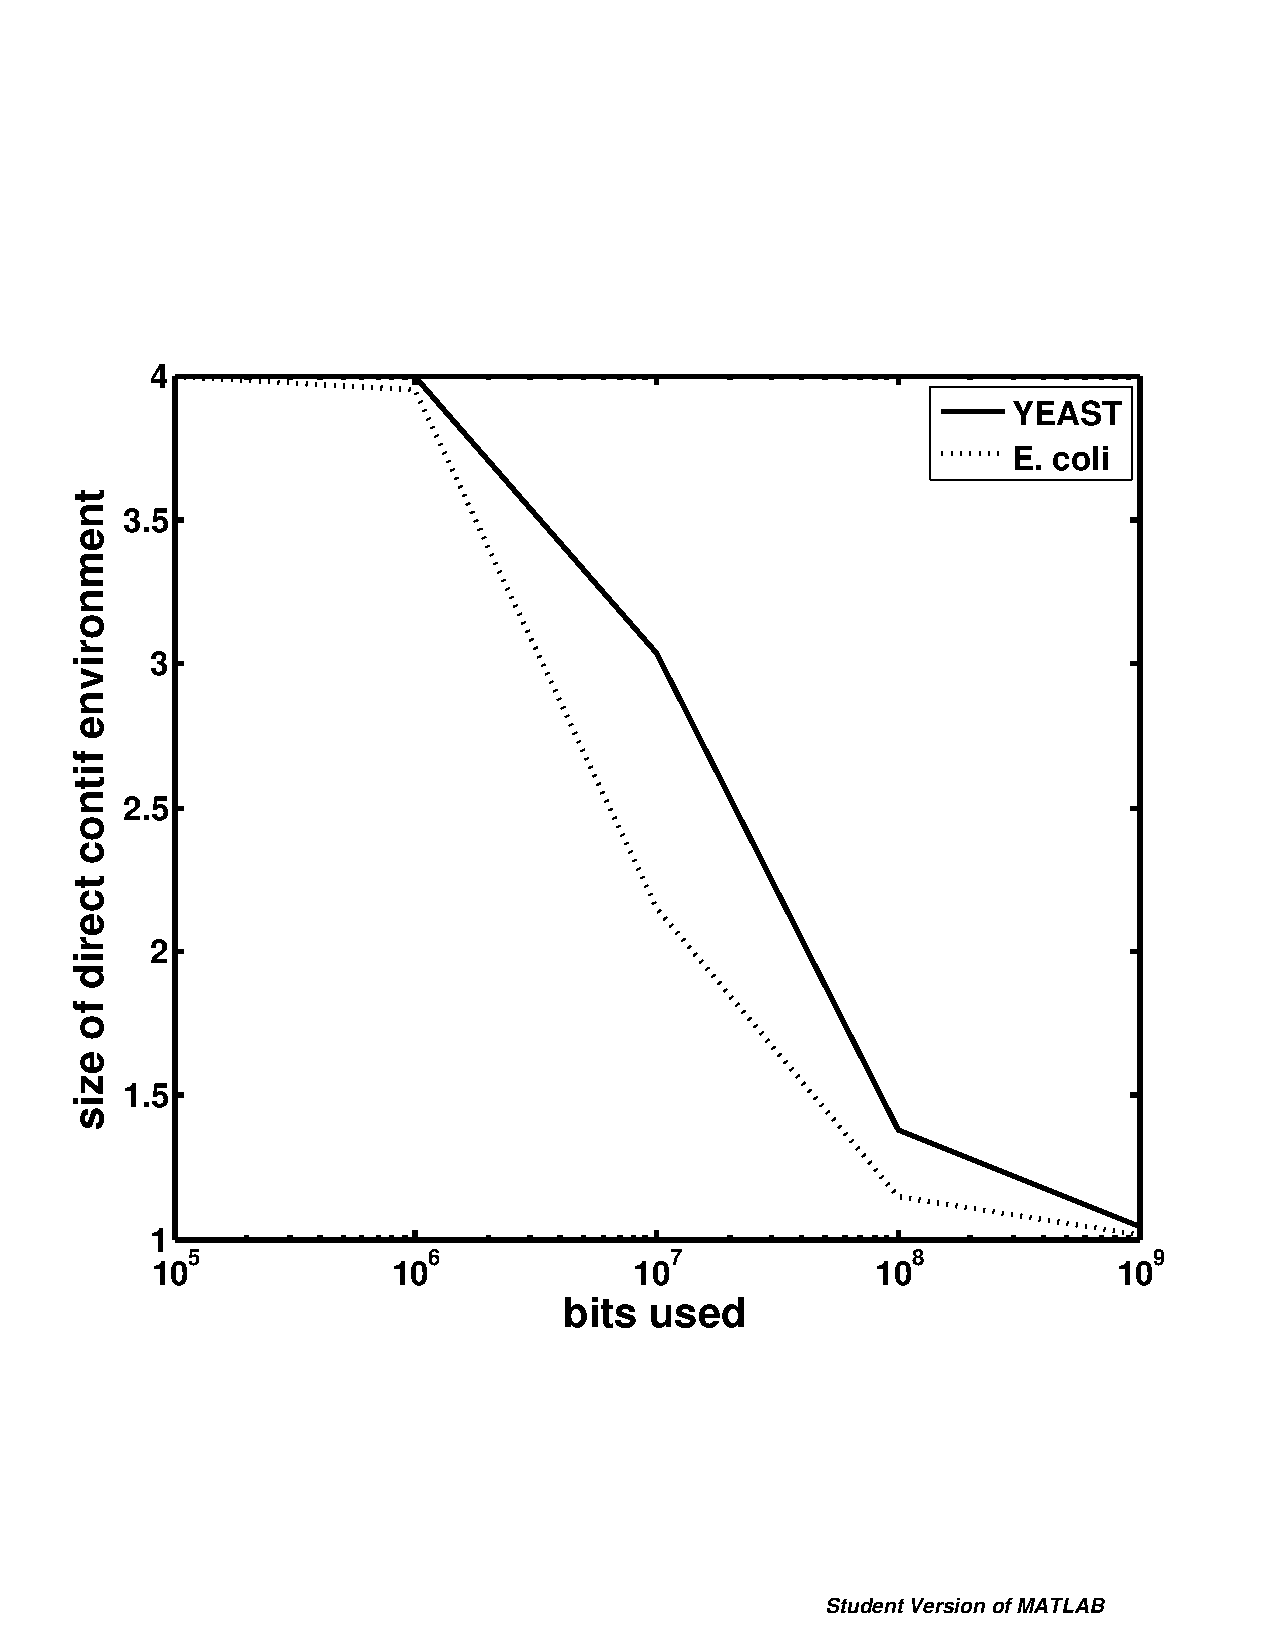
\includegraphics[width=5in]{contigEnvironment}}
\caption{Number of false connections introduced by inexact k-mer storage.
k = ??}
\end{figure}

\begin{figure}
\center{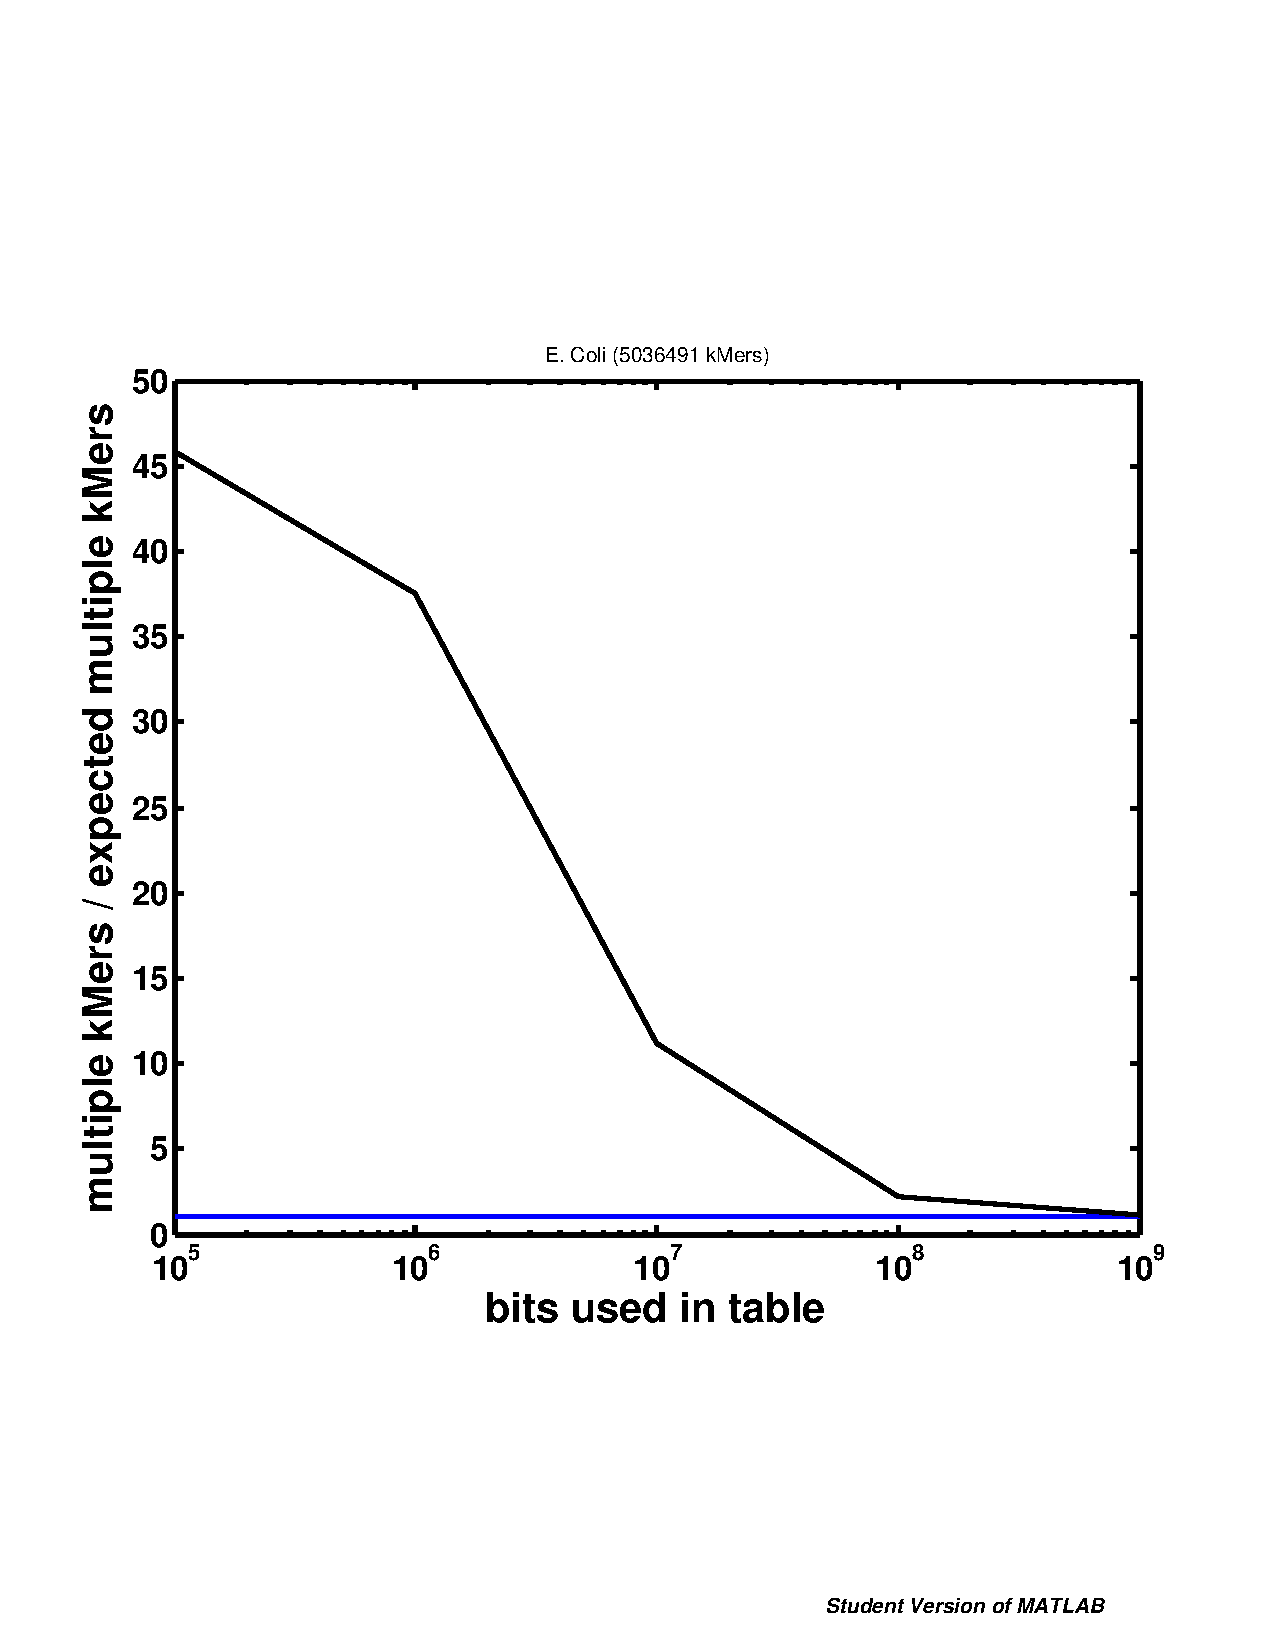
\includegraphics[width=5in]{fractionOfFoundDoubleHitsECOLI}}
\caption{The difference between exact and inexact kmer storage for the
ecoli genome. k = ??}
\end{figure}

\begin{figure}
\center{\includegraphics[width=5in]{fractionOfFoundDoubleHitsYEAST}}
\caption{The difference between exact and inexact kmer storage for the
yeast genome. k = ??}
\end{figure}

Idea for last graph:

We would do an exact representation of the E.coli genome, an exact 
representation of an Illumina dataset for E.coli, and then inexact
representations for each with different false positive rates (1\% and
10\%). We can then compare the exact genome versus other types to see
how the number of unique kmers, the number of duplicate kmers, and the
average neighbors per vertex changes. Ultimately, we would be able to
argue that the number of erroneous k-mers created by Illumina
sequencing eclipses that of what is created using our approach.

\end{document}
